% This LaTeX was auto-generated from MATLAB code.
% To make changes, update the MATLAB code and export to LaTeX again.

\documentclass{article}

\usepackage[utf8]{inputenc}
\usepackage[T1]{fontenc}
\usepackage{lmodern}
\usepackage{graphicx}
\usepackage{color}
\usepackage{hyperref}
\usepackage{amsmath}
\usepackage{amsfonts}
\usepackage{epstopdf}
\usepackage[table]{xcolor}
\usepackage{matlab}

\sloppy
\epstopdfsetup{outdir=./}
\graphicspath{ {./reporte_solucion_images/} }

\matlabmultipletitles

\begin{document}

\matlabtitle{Solución de Taller Filtros}

\begin{par}
\begin{flushleft}
En este taller practicaremos el desarrollo de filtros en tiempo continuo. Al final realizaremos una aplicación de estos filtros par amejorar la calidad de una señal de electrocardiograma (ECG).
\end{flushleft}
\end{par}

\matlabtitle{Punto I: Diseño de un filtro pasabanda y rechaza banda.}

\begin{itemize}
\setlength{\itemsep}{-1ex}
   \item{\begin{flushleft} Diseñe un filtro pasabanda cuyas frecuencias de corte son $\omega_1 =1000*2*\pi$, y $\omega_2 =2000*2*\pi$. Trate que la respuesta sea lo mas cercana a la respuesta ideal (forma rectangular en su amplitud). \end{flushleft}}
\end{itemize}

\matlabheadingtwo{Para completar este punto tomamos varias aproximaciones:}

\matlabheadingtwo{ }

\begin{par}
\begin{flushleft}
Antes de explicar a profundidad cada una de estas aproximaciones es importante hablar de algunas generalidades, para completar esta primera tarea hicimos una función que se encarga de producir la respuesta en frecuencia dadas las ubicaciones de los polos y los zeros ( '\textit{compute\_rect\_window.m' }). 
\end{flushleft}
\end{par}

\begin{par}
\begin{flushleft}
Con esta función probamos los límites de nuestra idea inicial: agregar un número arbitrariamente alto de polos en el intervalo que queremos dejar pasar con nuestro pasabandas, y un número también grande de zeros a los lados, donde no queríamos dejar pasar nada, los resultados fueron un vector de NAN o INF, esto porque el cálculo de las magnitudes de la rta. en frec. se hace tremendamente grande con tantos polos y zeros.
\end{flushleft}
\end{par}

\begin{par}
 $$H\left(j\omega \right)=k\cdot \;\frac{\;\prod_{i=1} \left(j\omega -z_i \right)}{\prod_{i=1} \left(j\omega -p_i \;\right)}$$
\end{par}


\vspace{1em}
\begin{par}
\begin{flushleft}
La enseñanza inicial fue entonces empezar a poner menos polos y menos zeros, y usarlos más sabiamente.
\end{flushleft}
\end{par}

\begin{par}
\begin{flushleft}
Con ello:
\end{flushleft}
\end{par}

\matlabheadingthree{Método 1:}


\begin{matlabcode}
%% inicialización de variables necesarias

L = 180000; %Longitud de la señal
T = 30;     %Duración de la señal
Fs = L/T;   %Frecuencia de muestreo

%vector entre 0 y 1/2 multiplicado por Fs
%vector entre 0 y Fs/2
f = Fs*(0:L/2)/L;

%vector de tiempo de 10000 elementos
t = linspace(0, T, L);
y = sin(2*pi*t);        %señal sinusoidal
w = f*2*pi;             %vector omega, de frecuencias angulares
epsilon = 0.00000000001;
\end{matlabcode}


\begin{par}
\begin{flushleft}
Para usar bien estos \textbf{ceros} nos dimos cuenta de que poner todos los ceros justo en el origen no es tan buena idea si queremos obtener una respuesta más suavizada respecto al punto en que dejan dehaber zeros y empiezan a haber polos y viceversa. \textit{(frecuencias de corte).}
\end{flushleft}
\end{par}


\begin{matlabcode}
%distanciamiento de la parte real de los ceros siguiendo una distrib
%logarítmica 

realPart1 = [ log( linspace(0 + epsilon, 999, 7) )]; 
zeros1 = [ linspace(0, 999, 7)*2*pi ].*1i - realPart1; 
\end{matlabcode}


\begin{matlabcode}
%distanciamiento de la parte real de los ceros siguiendo una distrib
%logarítmica inversa

realPart2 = [ log( linspace(2001, 3000,7) ).^-1 ];
zeros2 = [ linspace(2001, 3000,7)*2*pi ].*1i - realPart2;

zeros = [zeros1 zeros2];
\end{matlabcode}


\begin{matlabcode}
%finalmente tuning manual para la parte real de los polos 
Realpart3 = [0.00001  0.05  0.001  0.1  1  1  1  1  1  0.1  0.1  0.001  0.001 0.000001];

poles = [ linspace(1000, 2000, 14)*2*pi ].*1i-Realpart3;
% creación de la respuesta en freq
H_H  = compute_rect_window(w,poles,zeros);

plot_all_about_win(f, t, H_H, 'Filtro pasa banda por método 1');
\end{matlabcode}
\begin{center}
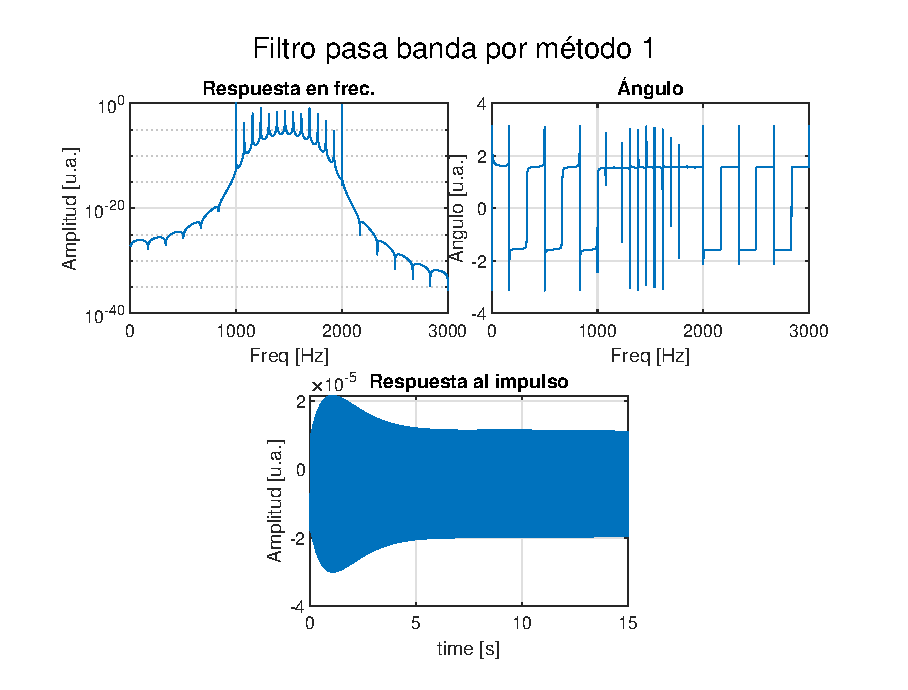
\includegraphics[width=\maxwidth{56.196688409433015em}]{figure_0.eps}
\end{center}


\vspace{1em}

\matlabheadingthree{Resultados método 1: }


\vspace{1em}
\begin{matlabcode}
H_H_C = [H_H(1:end-1) conj( fliplr(H_H(2:end)) ) ]; %flip left to right
y_filtered = plot_sys_output(y, t,  H_H_C); 
title('Resultado de la ventana por método 1')
\end{matlabcode}
\begin{center}
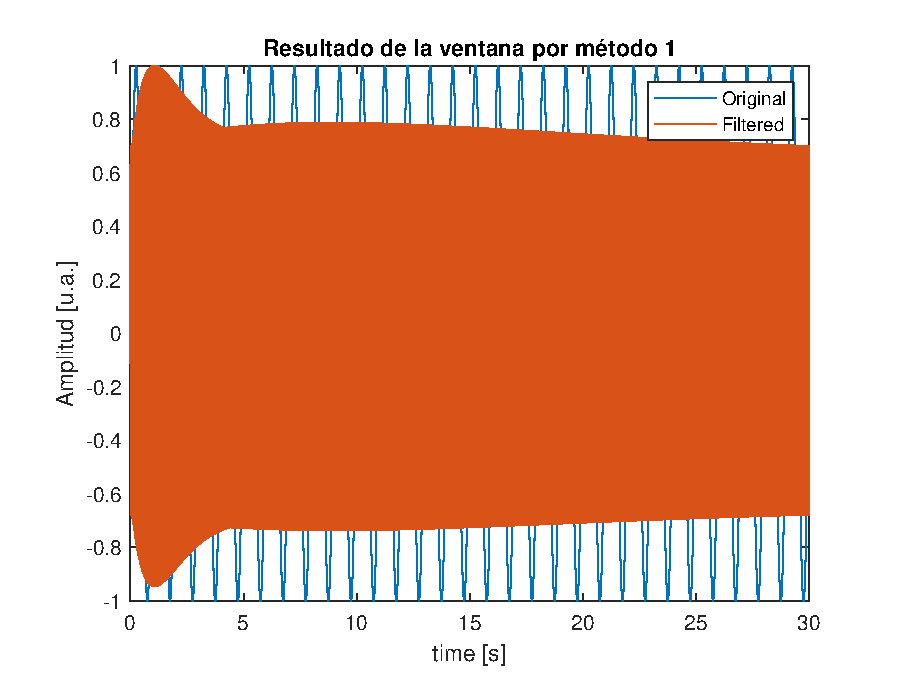
\includegraphics[width=\maxwidth{56.196688409433015em}]{figure_1.eps}
\end{center}


\begin{par}
\begin{flushleft}
También recordamos que en clases se mencionó que un filtro pasa bandas se hace pasando la señal por un pasa altas y después por un pasa bajas, esto combinado con la idea de poner solo \textit{ceros} y un polo = 1 es el otro método que probamos. 
\end{flushleft}
\end{par}


\vspace{1em}
\matlabheadingthree{Método 2: }


\vspace{1em}
\begin{par}
\begin{flushleft}
1. Filtro pasa altas
\end{flushleft}
\end{par}


\vspace{1em}
\begin{matlabcode}
dist_max = 600;

%parte real de los ceros del pasabajas
realPart1 = [ log(linspace(0 + epsilon, dist_max, 20) ) ]; 
zeros1 = [ linspace(0, dist_max, 20)*2*pi ].*1i - realPart1; 

H_H1 = high_pass_win(w, 1, zeros1);
plot_all_about_win(f, t, H_H1, 'Filtro pasa altas');
\end{matlabcode}
\begin{center}
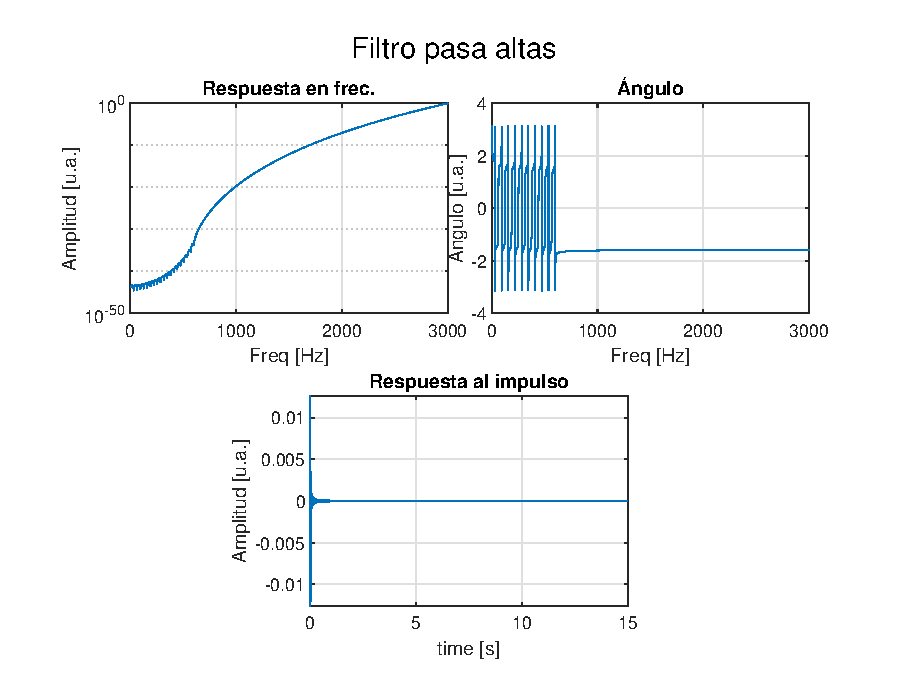
\includegraphics[width=\maxwidth{56.196688409433015em}]{figure_2.eps}
\end{center}


\begin{par}
\begin{flushleft}
2. Filtro pasa bajas
\end{flushleft}
\end{par}


\vspace{1em}
\begin{matlabcode}
realPart2 = [ log(linspace(3000-dist_max, 3000, 30) + epsilon) ]; 
zeros2 = [ linspace(3000-dist_max, 3000, 30)*2*pi ].*1i %- realPart2; 
\end{matlabcode}
\begin{matlaboutput}
zeros2 = 1x30 complex    
1.0e+04 *

   0.0000 + 1.5080i   0.0000 + 1.5210i   0.0000 + 1.5340i   0.0000 + 1.5470i   0.0000 + 1.5600i   0.0000 + 1.5730i   0.0000 + 1.5860i   0.0000 + 1.5990i   0.0000 + 1.6120i   0.0000 + 1.6250i   0.0000 + 1.6380i   0.0000 + 1.6510i   0.0000 + 1.6640i   0.0000 + 1.6770i   0.0000 + 1.6900i   0.0000 + 1.7030i   0.0000 + 1.7160i   0.0000 + 1.7290i   0.0000 + 1.7420i   0.0000 + 1.7550i   0.0000 + 1.7680i   0.0000 + 1.7810i   0.0000 + 1.7940i   0.0000 + 1.8070i   0.0000 + 1.8200i   0.0000 + 1.8330i   0.0000 + 1.8460i   0.0000 + 1.8590i   0.0000 + 1.8720i   0.0000 + 1.8850i

\end{matlaboutput}
\begin{matlabcode}

H_H2 = high_pass_win(w, 1, zeros2);
plot_all_about_win(f, t, H_H2, 'Filtro pasa bajas');
\end{matlabcode}
\begin{center}
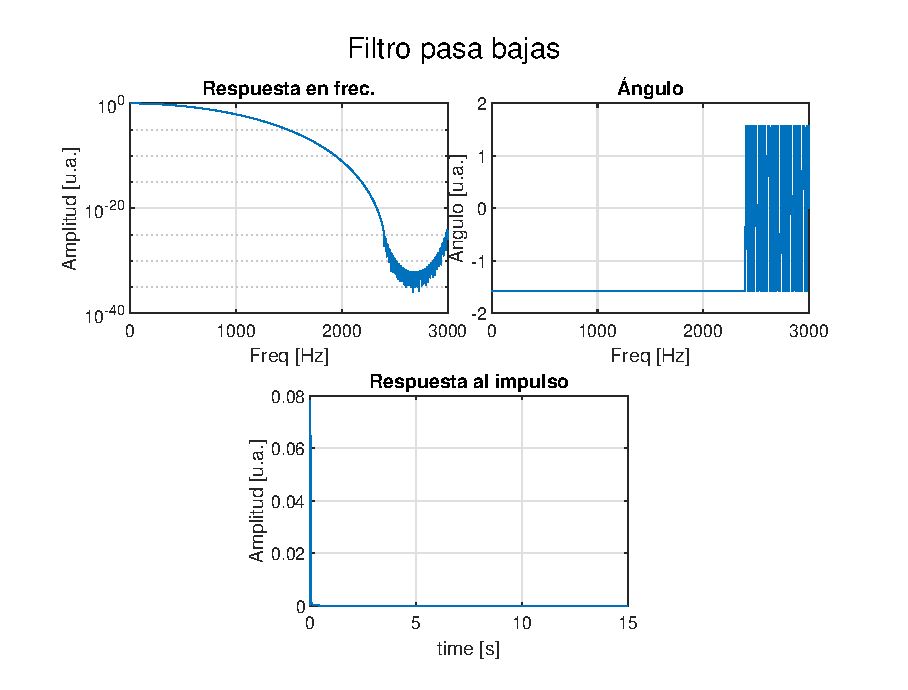
\includegraphics[width=\maxwidth{56.196688409433015em}]{figure_3.eps}
\end{center}


\begin{par}
\begin{flushleft}
3. Filtro conjunto
\end{flushleft}
\end{par}


\vspace{1em}
\begin{matlabcode}
H_H = (H_H1.*H_H2);
H_H = H_H./max(abs(H_H));
plot_all_about_win(f, t, H_H, 'Filtro pasa banda por método 2');
\end{matlabcode}
\begin{center}
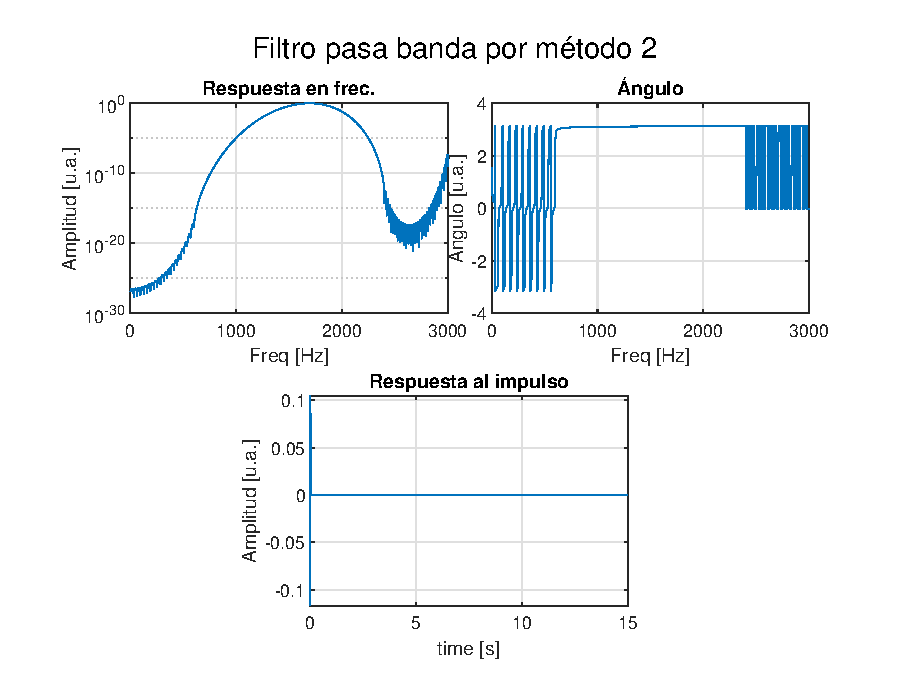
\includegraphics[width=\maxwidth{56.196688409433015em}]{figure_4.eps}
\end{center}


\matlabheadingtwo{Resultados método 2:}


\vspace{1em}
\begin{matlabcode}
H_H_C = [H_H(1:end-1) conj( fliplr(H_H(2:end)) ) ]; %flip left to right
y_filtered = plot_sys_output(y, t,  H_H_C); 
title('Resultado de la ventana por método 2')
\end{matlabcode}
\begin{center}
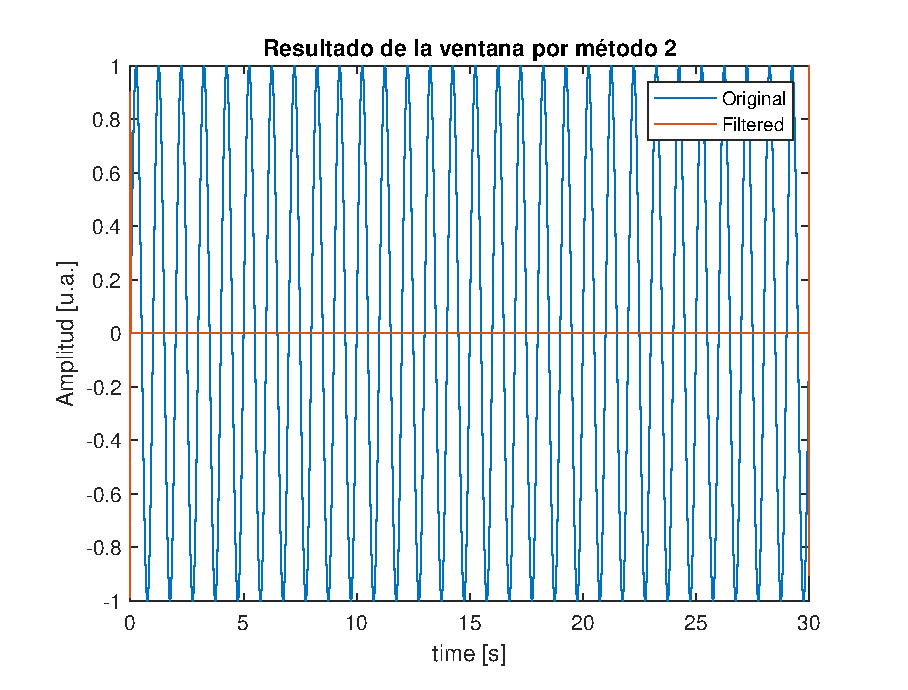
\includegraphics[width=\maxwidth{56.196688409433015em}]{figure_5.eps}
\end{center}


\matlabheadingthree{Método 3:}


\vspace{1em}
\begin{par}
\begin{flushleft}
Consiste en poner los polos y los ceros muy lejos del eje de las frecuencias para que se vea más suave la respuesta en frecuencia, aquí se entienden los ceros como un \textit{'contrapeso'} de los polos en el denominador, aunque acercando estos últimos al eje de frecuencias podemos generar un efecto de \textit{'levantamiento suave'} que puede resultar muy útil.
\end{flushleft}
\end{par}


\vspace{1em}
\begin{matlabcode}
dist = 10000;

zeros1 = [linspace(1000, 2000, 10)].*(2*pi*1i) - dist*500;
zeros2 = [linspace(1000, 2000, 10)].*(2*pi*1i) - dist*100000;
%zeros3 = [linspace(2000, 3000, 5)].*(2*pi*1i) - dist*100000;
zeros = [zeros1 zeros2] %zeros3];
\end{matlabcode}
\begin{matlaboutput}
zeros = 1x20 complex    
1.0e+09 *

  -0.0050 + 0.0000i  -0.0050 + 0.0000i  -0.0050 + 0.0000i  -0.0050 + 0.0000i  -0.0050 + 0.0000i  -0.0050 + 0.0000i  -0.0050 + 0.0000i  -0.0050 + 0.0000i  -0.0050 + 0.0000i  -0.0050 + 0.0000i  -1.0000 + 0.0000i  -1.0000 + 0.0000i  -1.0000 + 0.0000i  -1.0000 + 0.0000i  -1.0000 + 0.0000i  -1.0000 + 0.0000i  -1.0000 + 0.0000i  -1.0000 + 0.0000i  -1.0000 + 0.0000i  -1.0000 + 0.0000i

\end{matlaboutput}
\begin{matlabcode}

poles1 = [linspace(1000, 2000, 5)].*(2*pi*1i) - dist*1000/(dist);
poles2 = [linspace(2000, 3000, 6)].*(2*pi*1i) - dist*1000/(dist);

poles3 = [linspace(600, 1000, 2)].*(2*pi*1i) - dist*1200/(dist);


poles = [poles1 poles2 poles3 (1000.*(2*pi*1i) - dist*20000/(dist))  ];

plot_poles_and_zeros(poles, zeros)
\end{matlabcode}
\begin{center}
\includegraphics[width=\maxwidth{56.196688409433015em}]{figure_6.eps}
\end{center}
\begin{matlabcode}

H_H = compute_rect_window(w, poles, zeros);
ang = angle(H_H);
plot_all_about_win(f, t, H_H, 'Filtro pasa altas');
\end{matlabcode}
\begin{center}
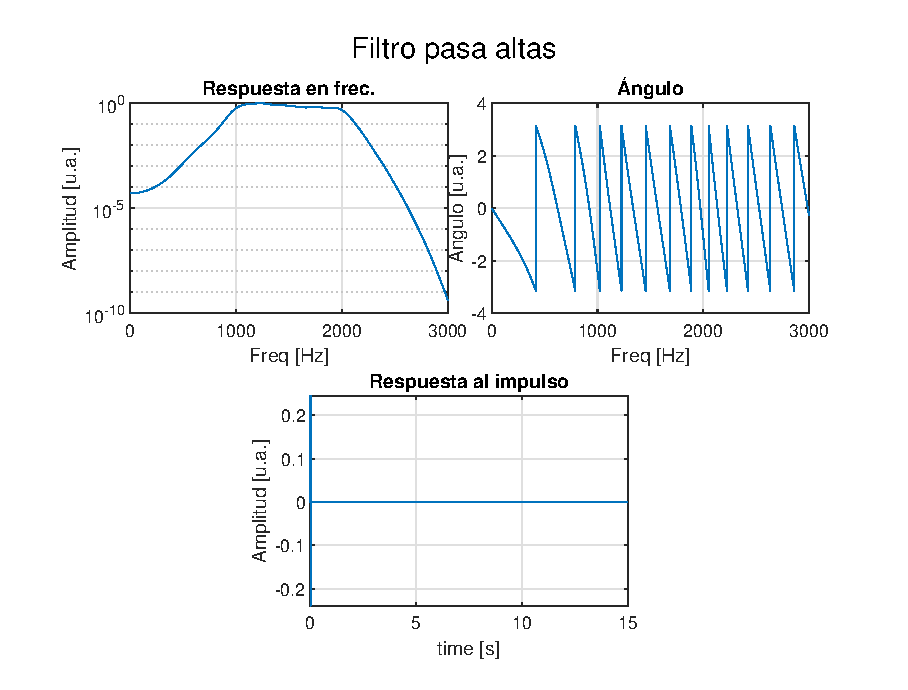
\includegraphics[width=\maxwidth{56.196688409433015em}]{figure_7.eps}
\end{center}



\vspace{1em}


\vspace{1em}
\matlabheadingtwo{Resultados método 3:}


\vspace{1em}
\begin{matlabcode}
H_H_C = [H_H(1:end-1) conj( fliplr(H_H(2:end)) ) ]; %flip left to right
y_filtered = plot_sys_output(y, t,  H_H_C); 
title('Resultado de la ventana por método 3')
\end{matlabcode}
\begin{center}
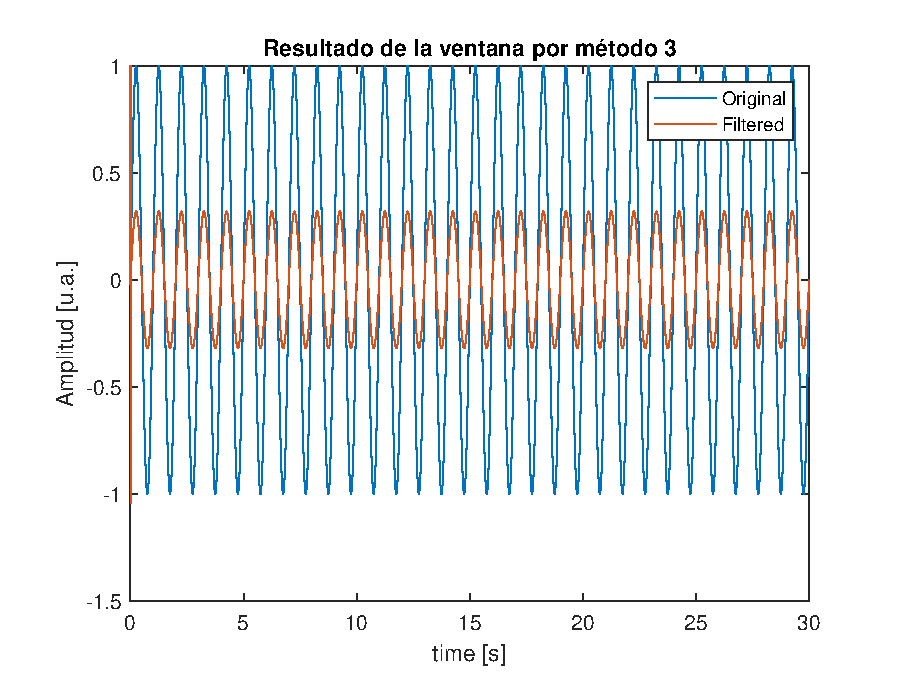
\includegraphics[width=\maxwidth{56.196688409433015em}]{figure_8.eps}
\end{center}


\vspace{1em}
\begin{par}
\begin{flushleft}
Usando un truco para construir el rechazabanda a partir del pasa banda anterior se tiene: 
\end{flushleft}
\end{par}


\vspace{1em}
\begin{matlabcode}
H_H_esp = 1 - abs(compute_rect_window(w, poles, zeros));
H_H = H_H_esp.*exp(ang.*1i);
figure, plot(f, abs(H_H) );
xlabel('frec. [Hz]')
ylabel('Amplitud [u.a.]')
title('Rechazabanda trucazo (No semilogy)')
\end{matlabcode}
\begin{center}
\includegraphics[width=\maxwidth{56.196688409433015em}]{figure_9.eps}
\end{center}
\begin{matlabcode}

plot_all_about_win(f, t, H_H, 'Filtro rechaza banda');
\end{matlabcode}
\begin{center}
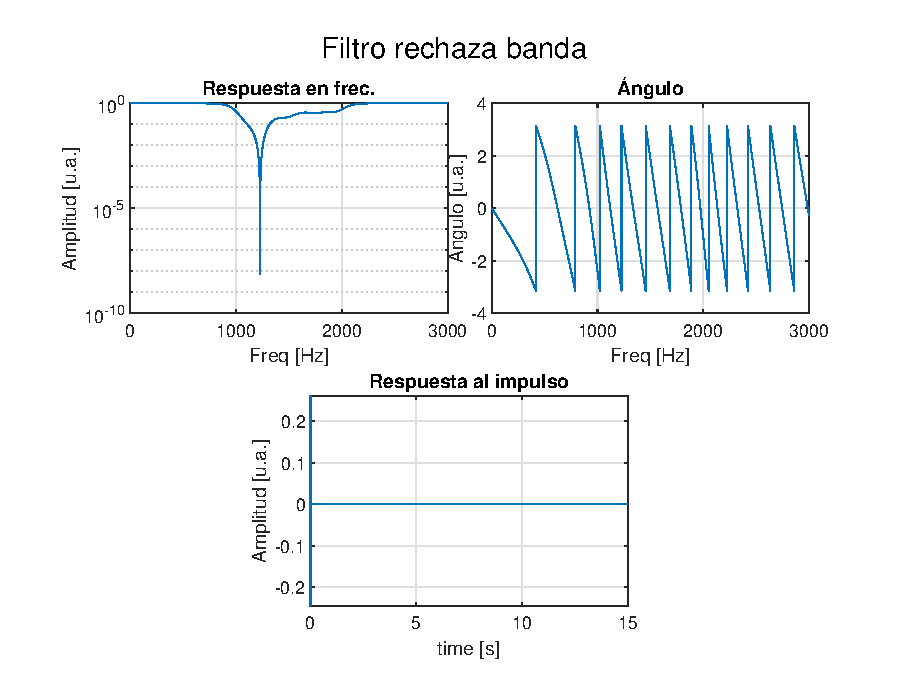
\includegraphics[width=\maxwidth{56.196688409433015em}]{figure_10.eps}
\end{center}


\vspace{1em}


\vspace{1em}
\begin{itemize}
\setlength{\itemsep}{-1ex}
   \item{\begin{flushleft} Utilizando las mismas frcuencias de corte realice un filtro rechaza banda. También trate de que la respuesta sea lo mas cercana a la respuesta ideal. \end{flushleft}}
\end{itemize}

\matlabheadingtwo{Para completar este punto tomamos varias aproximaciones:}


\vspace{1em}
\matlabheadingthree{1. Usando ceros y polos:}


\vspace{1em}
\begin{matlabcode}
%realPart1 = [ log(linspace(0 + epsilon, dist_max, 20) ) ]; 
zeros1 = [ linspace(1000, 2000, 20)*2*pi ].*1i ; 

poles = [1  2000].*(2*pi*1i) - [1 1000000];

H_H1 = compute_rect_window(w, poles, zeros1);
plot_all_about_win(f, t, H_H1, 'Filtro rechaza bandas');
\end{matlabcode}
\begin{center}
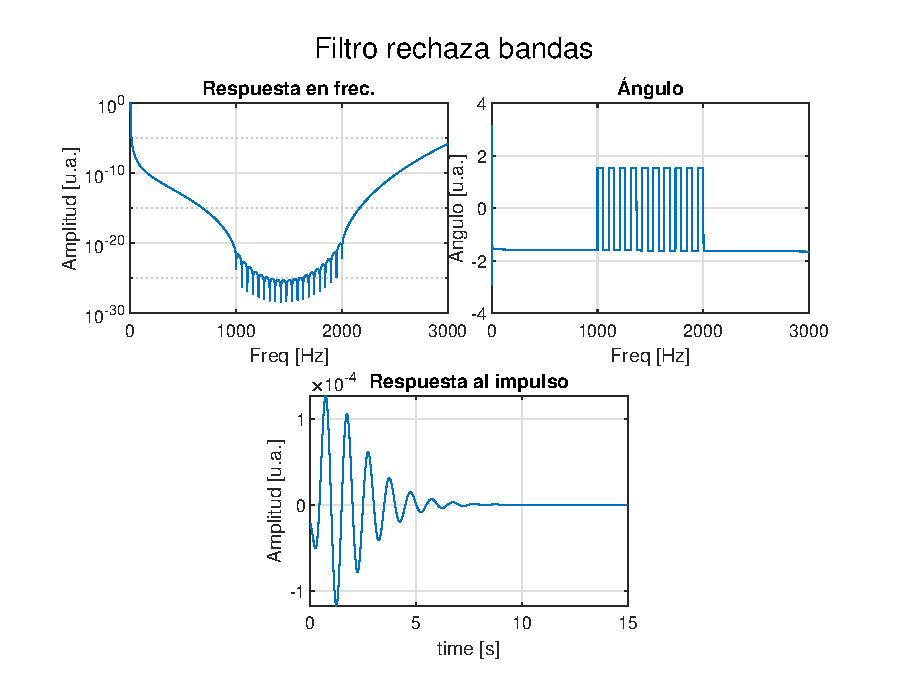
\includegraphics[width=\maxwidth{56.196688409433015em}]{figure_11.eps}
\end{center}



\vspace{1em}
\begin{matlabcode}
dist = 10000;
zeros = [linspace(1000, 2000,4)].*(2*pi*1i) + dist;
poles = [linspace(1100, 3300,10)].*(2*pi*1i) + dist;

H_H1 = compute_rect_window(w, poles, zeros);
plot_all_about_win(f, t, H_H1, 'Filtro pasa bajas');
\end{matlabcode}
\begin{center}
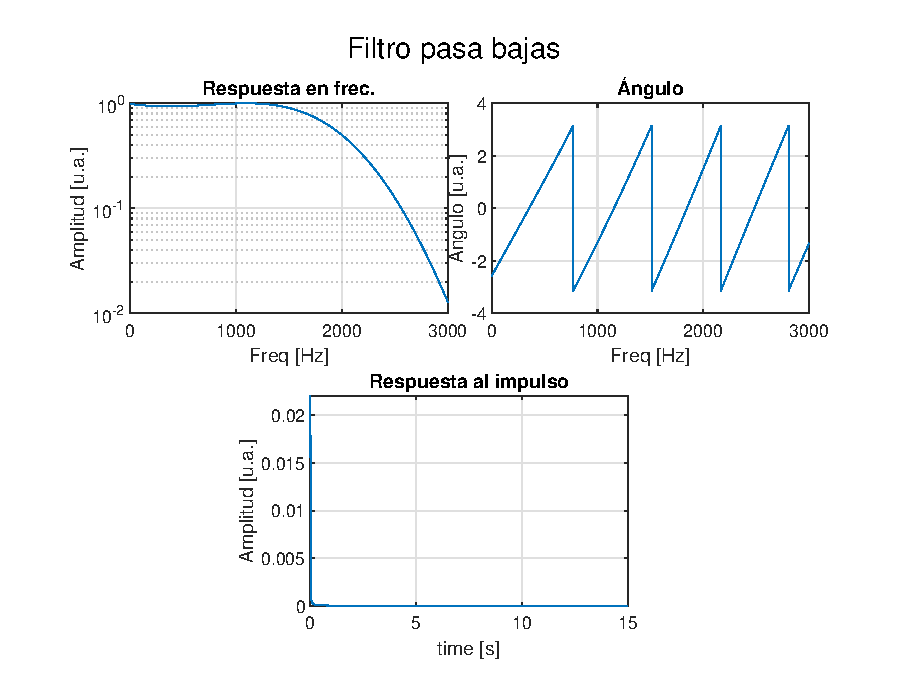
\includegraphics[width=\maxwidth{56.196688409433015em}]{figure_12.eps}
\end{center}



\vspace{1em}
\begin{matlabcode}

\end{matlabcode}


\vspace{1em}
\vspace{1em}

\end{document}
